
\subsection{Estimated transitions}
Figure~\ref{fig:transitions} shows two of the 84 estimated transition matrices, for attacking players aged 23 to 25. The diagonal dominates: careers are persistent from one quarter to the next. The talent tier changes the picture in the upper states. A Strong player of the top tier stays Strong with probability 0.70, whereas in the bottom tier the Strong state is fragile and players fall back to Starter or Rotation. Injured players mostly return through Rotation, as one would expect of a player regaining fitness.

\begin{figure}[h]
\centering
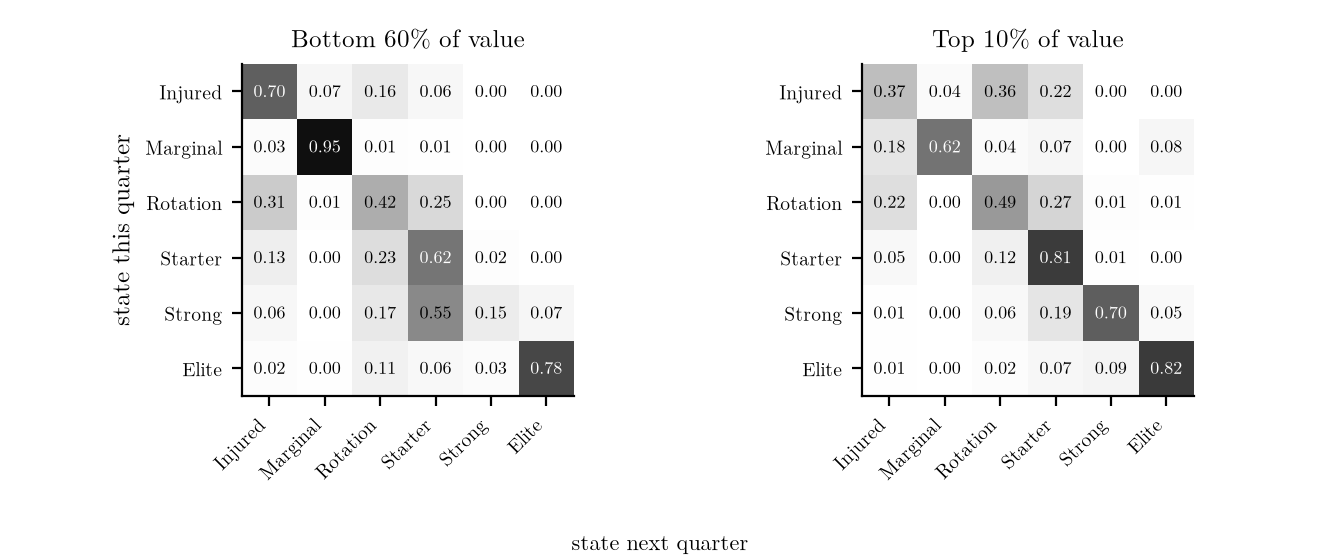
\includegraphics[width=\textwidth]{figures/transitions.png}
\caption{Estimated quarterly transition matrices for attacking players aged 23--25.}
\label{fig:transitions}
\end{figure}

The Elo ratings computed with the conservation rule of Proposition~\ref{prop:elo} order the five leagues consistently over time (Figure~\ref{fig:elo}).

\begin{figure}[h]
\centering
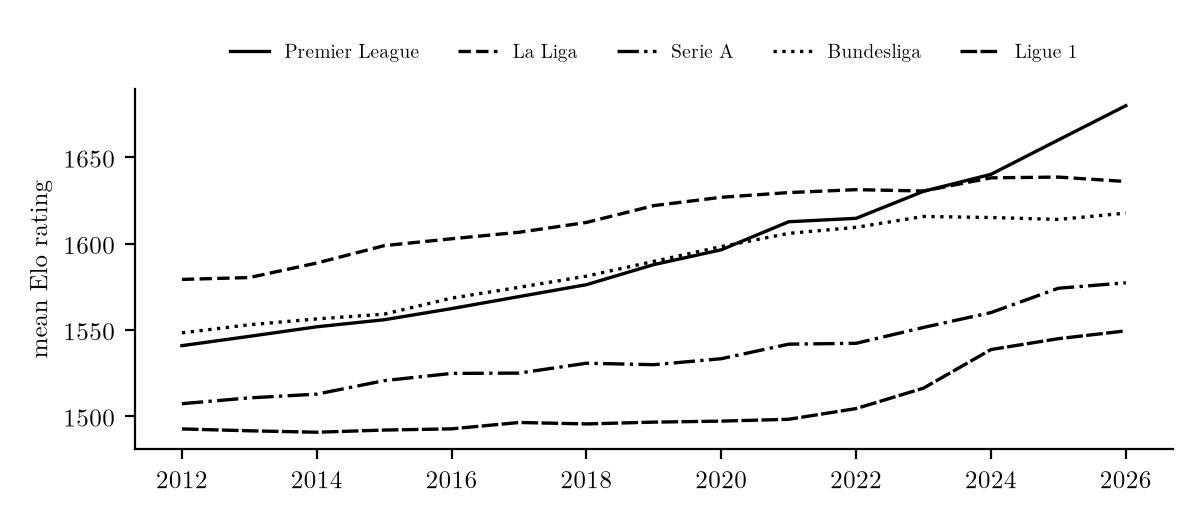
\includegraphics[width=0.92\textwidth]{figures/elo.png}
\caption{Mean Elo rating of clubs in the five major leagues.}
\label{fig:elo}
\end{figure}

\subsection{An example: Bukayo Saka}
Bukayo Saka was 25.2 years old at the start of the forecast and valued at 110 million euros. The on-demand update downloads his 7 league matches of 2026/27: he played 83\% of available minutes in August--October, then disappeared from every team sheet, which the model reads as an injury. His starting distribution is therefore 100\% Injured. Figure~\ref{fig:example} shows the result of $10\,000$ simulated careers. The median real value is 104 million euros after one year, 92 after three and 42 after six, with an 80\% interval of 20 to 74 million euros in 2032. The probability that he is worth at least 100 million euros four years from now is 26\%. The right panel shows the mechanism: most careers leave the Injured state within two quarters, and the share of Strong and Elite quarters slowly declines as he moves past 28.

\begin{figure}[h]
\centering
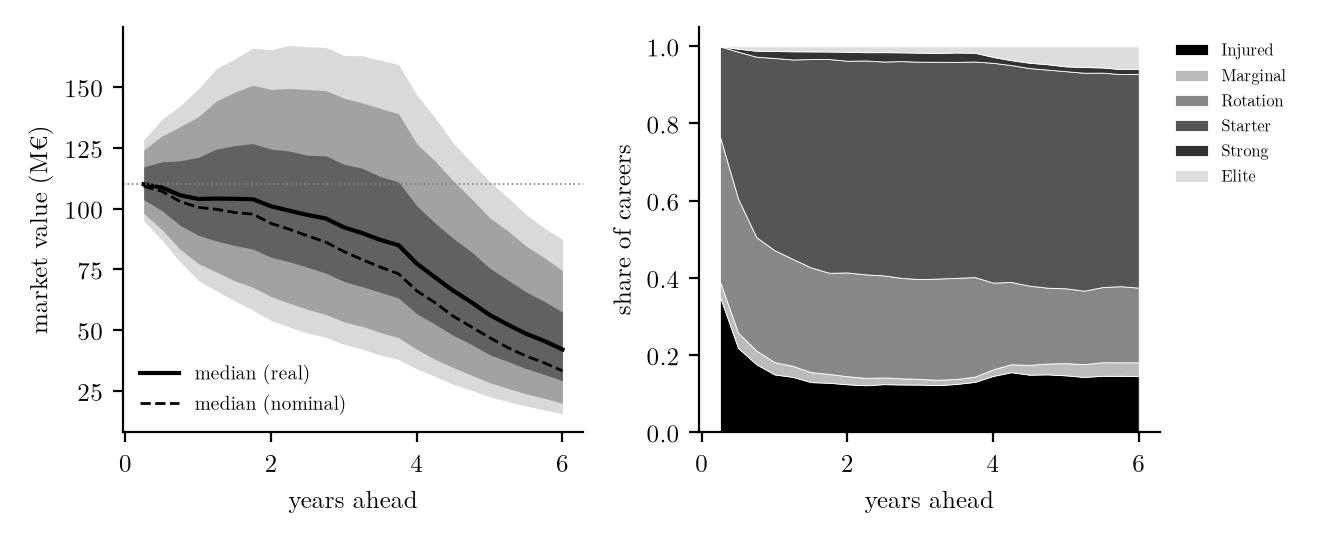
\includegraphics[width=\textwidth]{figures/example.png}
\caption{Bukayo Saka: distribution of simulated market values (left; bands contain 50\%, 80\% and 90\% of careers) and of latent states (right).}
\label{fig:example}
\end{figure}

\subsection{Out-of-sample validation}
A model of this kind can always be made to look plausible on a few famous names. The only honest test is to forecast the past. We therefore placed ourselves in July 2020: every component (the hidden Markov model, the valuation equations, the event probabilities, the team-contribution model and the drift calibration) was re-estimated with data available at that date only. We then simulated six years ahead for 358 players of the top five leagues, aged 18 to 32 and worth at least one million euros, stratified by value, and compared the forecasts with their true Transfermarkt values in June 2026.

Three numbers summarise a probabilistic forecast. The \emph{coverage} of the 80\% interval should be close to 80\%. The \emph{bias} is the mean of $\log(\text{forecast median}/\text{truth})$, ideally zero. The \emph{PIT} is the fraction of simulated careers below the true value; if the forecasts are well calibrated it is uniformly distributed, with mean $0.5$. Table~\ref{tab:backtest} shows how the model improved as its flaws were found and corrected. In reality the median player kept only 0.29 of his 2020 value six years later; the naive simulation predicted 0.81.

\begin{table}[h]
\centering
\begin{tabular}{lcccc}
\toprule
Model & value ratio 2026/2020 & 80\% coverage & bias (log) & mean PIT \\
\midrule
Naive simulation & 0.81 & 63\% & +0.99 & 0.24 \\
+ league changes, yearly talent tier & 0.70 & 70\% & +0.90 & 0.28 \\
+ drift calibration & 0.39 & 83\% & +0.22 & 0.45 \\
\textbf{+ FotMob xG, defence and injuries (final)} & \textbf{0.30} & \textbf{80\%} & \textbf{-0.03} & \textbf{0.51} \\
\midrule
True outcome & 0.29 & 80\% & 0 & 0.50 \\
\bottomrule
\end{tabular}
\caption{Out-of-sample forecasts from July 2020 to June 2026 (358 players).}
\label{tab:backtest}
\end{table}

The amount of market noise added in the simulation is the one free parameter of the forecast intervals. Table~\ref{tab:scale} shows the coverage for several values; we retain the value 0.25, whose 80\% interval covers the truth in 80\% of cases. The intervals are wide (the upper bound of the 80\% interval is on average 12 times the lower bound), which is the honest price of a six-year horizon: Raheem Sterling went from 128 to 3 million euros and Sadio Man\'e from 120 to 6 million between the two dates.

\begin{table}[h]
\centering
\begin{tabular}{ccccc}
\toprule
noise scale & 50\% coverage & 80\% coverage & 90\% coverage & width of 80\% interval (ratio) \\
\midrule
0.25 & 52\% & 80\% & 89\% & 12.3 \\
0.50 & 53\% & 82\% & 90\% & 13.8 \\
0.75 & 56\% & 85\% & 92\% & 16.3 \\
1.00 & 58\% & 87\% & 94\% & 20.5 \\
\bottomrule
\end{tabular}
\caption{Coverage of the forecast intervals as a function of the noise scale.}
\label{tab:scale}
\end{table}

Coverage is similar across value bands (Table~\ref{tab:bands}), but the bias changes sign: the model slightly overestimates the future value of players already worth more than 20 million euros and underestimates that of cheaper players. The overall bias is small only because these two errors largely cancel.

\begin{table}[h]
\centering
\begin{tabular}{lccc}
\toprule
value in 2020 & players & 80\% coverage & bias (log) \\
\midrule
$<$5\,M & 100 & 75\% & -0.24 \\
5-20\,M & 100 & 76\% & -0.09 \\
20-50\,M & 100 & 85\% & +0.16 \\
$>$50\,M & 58 & 84\% & +0.12 \\
\bottomrule
\end{tabular}
\caption{Validation by value band.}
\label{tab:bands}
\end{table}

\begin{figure}[h]
\centering
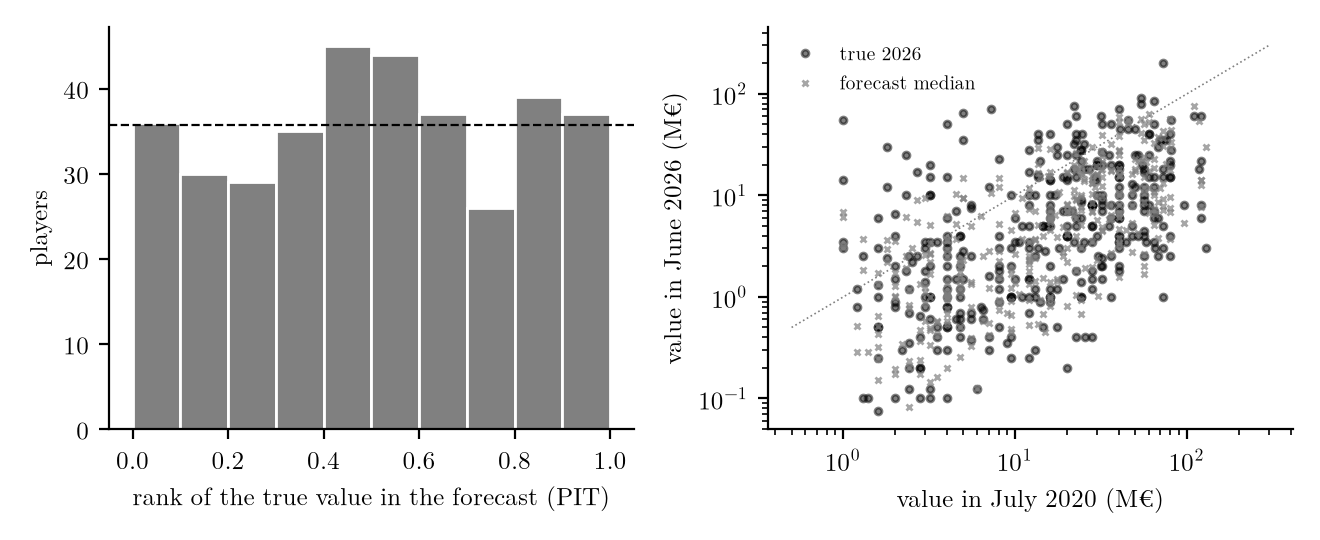
\includegraphics[width=\textwidth]{figures/backtest.png}
\caption{Out-of-sample validation. Left: the rank of the true value within the simulated distribution (a flat histogram means calibrated forecasts). Right: forecast medians and true values against the 2020 value.}
\label{fig:backtest}
\end{figure}
